\documentclass[11pt,aspectratio=169]{beamer}

% -------------------- THEME & LAYOUT --------------------
\usetheme{Madrid}
\usecolortheme{dolphin} % base color scheme
\usefonttheme{professionalfonts}
\setbeamercovered{transparent}
\setbeamertemplate{navigation symbols}{}   % remove navigation buttons
\setbeamertemplate{caption}[numbered]      % numbered captions
\setbeamertemplate{itemize items}[triangle]
\setbeamersize{text margin left=1.2cm,text margin right=1.2cm} % adjust to taste

% -------------------- GLOBAL FONT SETTINGS --------------------

% 1. Force the base beamer font to small
\setbeamerfont{normal text}{size=\small}

% 2. Force math environments to follow the "small" font size
\setbeamerfont{math text}{size=\small}
\setbeamerfont{equation}{size=\small}

% 3. Redefine \normalsize itself 
% This ensures equations and lists (which look for \normalsize) use  instead.
\let\oldnormalsize\normalsize
\renewcommand{\normalsize}{\oldnormalsize\small}

% 4. Ensure lists also stay small
\setbeamerfont{itemize/enumerate body}{size=\small}
\setbeamerfont{itemize/enumerate subbody}{size=\small}

% -------------------- FONTS & TYPOGRAPHY --------------------
\usepackage[T1]{fontenc}
\usepackage[utf8]{inputenc}
\usepackage{newpxtext,newpxmath} % Palatino-like font & math
\usepackage{microtype}

% -------------------- MATH, TABLES & GRAPHICS --------------------
\usepackage{amsmath,amssymb,amsfonts,mathtools}
\usepackage{bm,booktabs,siunitx,graphicx}
\graphicspath{{./}{./figures/}}
\renewcommand{\theequation}{7.\arabic{equation}}

% -------------------- UTILITIES --------------------
\usepackage{appendixnumberbeamer}
\usepackage{ragged2e}
\usepackage{xspace}
\usepackage{csquotes}
% -------------------- Bibliography --------------------
\usepackage[backend=biber,style=authoryear]{biblatex}
\addbibresource{sources.bib}
\usepackage{xcolor}

% -------------------- HYPERREF --------------------
\hypersetup{
  colorlinks=false,
  pdfauthor={Francesca},
  pdftitle={Chapter 1 — The Value of Currency}
}

% -------------------- COLORS & EMPHASIS --------------------
\definecolor{myblue}{RGB}{0,70,140}
\definecolor{myred}{RGB}{180,30,30}
\definecolor{mygreen}{RGB}{0,120,70}
\definecolor{gold}{RGB}{184,134,11}

\setbeamercolor{title}{fg=gold}       % title page
\setbeamercolor{frametitle}{fg=gold}  % slide titles
\setbeamercolor{structure}{fg=gold}   % bullets, sections, links
\setbeamercolor{section in head/foot}{fg=gold,bg=black!10} % gold text on light background

% -------------------- FOOTLINE --------------------
\setbeamertemplate{footline}{
  \leavevmode%
  \hbox{%
    % Section links (hidden if no current section)
    \begin{beamercolorbox}[wd=0.7\paperwidth,ht=2.5ex,dp=1.5ex,leftskip=1.4em]{section in head/foot}%
      \ifx\insertsection\empty
        % nothing
      \else
        Section: \insertsection
      \fi
    \end{beamercolorbox}%
    % Frame number right
    \begin{beamercolorbox}[wd=0.3\paperwidth,ht=2.5ex,dp=1.5ex,leftskip=3.8cm]{section in head/foot}%
      \insertframenumber/\inserttotalframenumber
    \end{beamercolorbox}%
  }%
  \vskip1pt%
}



\newcommand{\highlight}[1]{\textcolor{myblue}{#1}}
\newcommand{\warning}[1]{\textcolor{myred}{#1}}

% -------------------- SHORTCUTS --------------------
\newcommand{\E}{\mathbb{E}}
\newcommand{\R}{\mathbb{R}}
\newcommand{\dd}{\mathrm{d}}
\newcommand{\mc}[1]{\mathcal{#1}}
\newcommand{\bb}[1]{\mathbb{#1}}
\newcommand{\uc}{U_c}
\newcommand{\zg}{Z_g}

% -------------------- TIGHTER DISPLAY MATH --------------------
\makeatletter
\g@addto@macro\normalsize{%
  \setlength\abovedisplayskip{8pt}%
  \setlength\belowdisplayskip{8pt}%
  \setlength\abovedisplayshortskip{6pt}%
  \setlength\belowdisplayshortskip{6pt}%
}
\makeatother
\setbeamertemplate{frametitle}{
  \nointerlineskip
  \begin{beamercolorbox}[wd=\paperwidth,ht=3.5ex,dp=1ex,center]{frametitle}
    \centering\insertframetitle
  \end{beamercolorbox}
}

% -------------------- METADATA --------------------
\title[Part I — Currency and Money]{\textbf{Part I: Currency and Money}\\[2pt]\large Chapter 1 — The Value of Currency}
\subtitle{Currency, Money, and Price-Level Determination}
\author{Francesca}
\institute{}
\date{\today}

% -------------------- SECTION ROADMAP --------------------
\AtBeginSection[]
{
  \begin{frame}
    \tableofcontents[currentsection, hideothersubsections]
  \end{frame}
}


\begin{document}
\setcounter{equation}{0}


% ===================== TITLE SLIDE =====================
\begin{frame}[plain] % 'plain' removes header/footer for the title slide

\begin{columns}[T,totalwidth=\textwidth]

% ----- Left column: Main title, professor, chapter -----
\begin{column}{0.45\textwidth}
\vspace{2cm}

% Main title
{\usebeamercolor[fg]{title}\LARGE\textbf{Monetary Economics}\\[0.3cm]
\LARGE\textbf{and Policy}} 

\vspace{0.5cm}

% Professor name and date
{\large\textit{Pierpaolo Benigno}}\\[0.1cm]

\vspace{1cm}

% Chapter and subtitle
{\usebeamercolor[fg]{frametitle}\large Chapter 7: Inflation Targeting as an Optimal Policy}

\end{column}

% ----- Right column: Image -----
\begin{column}{0.55\textwidth}
\vspace{1cm}
\centering
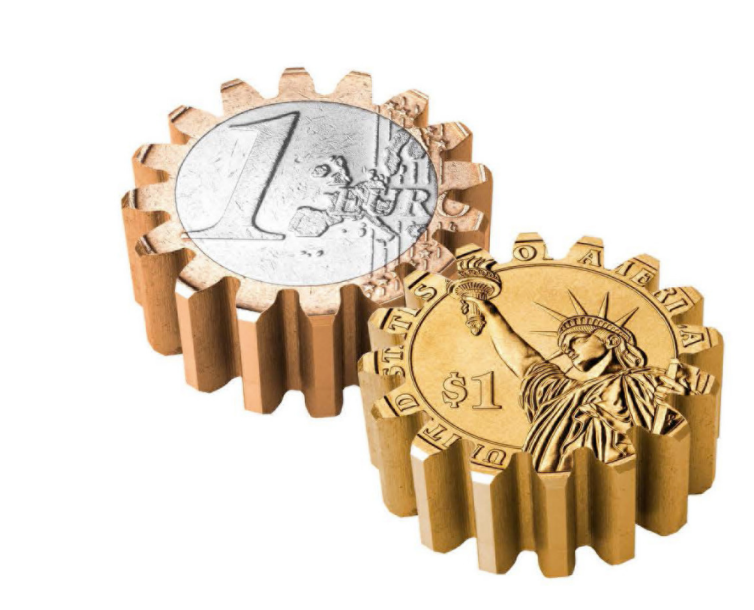
\includegraphics[width=0.9\linewidth]{Cover.png}
\end{column}

\end{columns}

% ----- Footer text (bottom-right corner) -----
\vspace*{2cm} % adjust if needed
\hfill{\large\textit{Prepared by Marcos Consuegra}}

\end{frame}


\begin{frame}{What We Will Learn}
\small
\begin{itemize}
  \item How the New Keynesian benchmark provides a theoretical foundation for \textbf{flexible inflation targeting} as an optimal policy strategy.
  \item How to derive the optimal targeting rule under \textbf{commitment} (specifically, the \textbf{timeless perspective}).
  \item How to distinguish optimal commitment from \textbf{discretion} and simple \textbf{interest-rate rules}, and how determinacy leads to the \textbf{Taylor principle}.
  \item How optimal policy under commitment introduces \textbf{history dependence} and \textbf{price-level reversion} to stabilize expectations.
  \item How to \textbf{rationalize and assess} the optimal numerical inflation target, and why many models imply a positive target in the \textbf{1--3\% range}.
\end{itemize}
\end{frame}


% OUTLINE
\begin{frame}{Outline}
\tableofcontents
\end{frame}

% ======================================================
\section{Introduction}

\begin{frame}{Inflation Targeting: Context and Theory}
\small

\textbf{Historical Context}
\begin{itemize}
  \item Pioneered by New Zealand (1990), followed by Canada, UK, Sweden, and Finland.
  \item US Federal Reserve formally adopted a 2\% target in 2012.
  \item \emph{Key Features:} Public announcement of a numerical target (typically 1--3\%) combined with central bank accountability.
\end{itemize}

\vspace{0.1cm}

\textbf{Theoretical Rationalization}
\begin{itemize}
  \item Practical implementation of inflation targeting strategies preceded the development of suitable academic frameworks.
  \item The New Keynesian benchmark provides the \textbf{microfoundations} that rationalize inflation targeting as the optimal policy regime.
  \item This approach proves superior to simple instrument rules or strict adherence to the Wicksellian natural rate ($r^\ast$).
\end{itemize}

\end{frame}

\begin{frame}[label=Loss Function]{Optimal Policy: The Welfare Criterion}
\small

\textbf{Microfounded Objective}
\begin{itemize}
  \item Policy evaluation is based on maximizing the household's expected utility.
  \item Since equilibrium conditions are log-linearized (first-order), a correct ranking of alternative policies requires a \textbf{second-order approximation} of utility.
\end{itemize}

\vspace{0.1cm}

\textbf{The Central Bank's Welfare-Based Loss Function}
\begin{equation}
L_{t_{0}}^{CB}
= \mathbb{E}_{t_{0}}\sum_{t=t_{0}}^{\infty}
\beta^{t-t_{0}}
\left[
\frac{1}{2}\big(\hat{Y}_{t}-\hat{Y}_{t}^{e}\big)^{2}
+ \frac{1}{2}\frac{\theta}{\kappa}\big(\pi_{t}-\pi\big)^{2}
\right]
\label{LossNK}
\end{equation}

\textbf{Definitions}
\begin{itemize}
  \item $\hat{Y}_{t}$: log deviation of output from steady state; $\hat{Y}_{t}^{e}$: \emph{efficient} level of output.
  \item $\pi_{t}$: inflation rate; $\pi$: inflation target.
  \item $\beta \in (0,1)$: households’ discount factor; $\theta>0$: elasticity of substitution across differentiated goods; $\kappa > 0$: slope of the New Keynesian Phillips curve.
\end{itemize}

\vspace{0.1cm}
\begin{center}
\hyperlink{Appendix F}{\beamerbutton{Derivation of Loss Function (Appendix)}}
\end{center}

\end{frame}

\begin{frame}{The Policy Problem: Objectives and Constraints}
\small

\textbf{Welfare-Theoretic Objective}
\begin{itemize}
  \item \textbf{Inflation stabilization:} Deviations $(\pi_t-\pi)$ create \emph{price dispersion}, implying an inefficient allocation of demand across otherwise identical goods.
  \item \textbf{Real activity:} The welfare-relevant output gap is measured relative to the \emph{efficient} level, $(\hat{Y}_t-\hat{Y}_t^{e})$, and deviations from efficiency are costly.
  \item \textbf{Relative weight:} The welfare-based loss function pins down the optimal weight on inflation stabilization versus output-gap stabilization (via $\theta/\kappa$).
  \item The loss is minimized when $\hat{Y}_t=\hat{Y}_t^{e}$ and $\pi_t=\pi$ \emph{simultaneously}.
\end{itemize}

\vspace{0.15cm}

\textbf{AS Constraint (New Keynesian Phillips Curve)}
\begin{equation}
\pi_t-\pi
= \kappa(\hat{Y}_t-\hat{Y}_t^{n}) + \beta\,\mathbb{E}_t(\pi_{t+1}-\pi),
\label{AS-7}
\end{equation}

\end{frame}


\begin{frame}{Nature of the Trade-off and Optimal Strategy}
\small

\textbf{Shocks and Trade-offs}
\begin{itemize}
  \item Following productivity or public spending shocks (\textbf{efficient shocks}), the natural rate $\hat{Y}_{t}^{n}$ coincides with the efficient level $\hat{Y}_{t}^{e}$.
  \item Optimal policy stabilizes inflation at the target and simultaneously closes the output gap.
  \item A trade-off arises \emph{only} with \textbf{markup shocks}, which create a wedge between the natural and efficient levels of output.
\end{itemize}

\vspace{0.3cm}

\textbf{Characterization of Optimal Policy}
\begin{itemize}
  \item \textbf{Flexible Inflation Targeting} balances deviations from price stability with corresponding variations in output gap growth.
  \item \textbf{Commitment} implies \textbf{history dependence}: deviations of prices from the target trend are gradually undone to revert prices to the initial trend.
\end{itemize}

\end{frame}

\section{Outline of the Results}
\begin{frame}{Outline of the Results}
\small

\begin{itemize}
    \item Under \textbf{commitment} (the timeless perspective), the optimal policy yields targeting rules that rationalize \textbf{flexible inflation targeting}.
    \item \textbf{Discretion} and simple interest-rate rules are proven \textbf{sub-optimal} relative to the commitment benchmark.
    \item The superiority of commitment stems from \textbf{policy inertia} (history dependence) and the property of \textbf{price-level reversion}.
    \item Analysis of the optimal \textbf{numerical value} for the inflation target $\pi$.
\end{itemize}

\end{frame}
% ====================================================

\section{Optimal policy under commitment}

\begin{frame}{Defining Optimal Policy under Commitment}
\small

\begin{itemize}
  \item \textbf{Commitment:} The policymaker chooses \emph{once and for all} a state-contingent path for the relevant macroeconomic variables and commits to implementing that plan in all future contingencies.

  \item \textbf{Not a Strict Rule:} Commitment does not imply adherence to a rigid instrument rule that is valid irrespective of the state of the economy. Instead, it consists of announcing and following an optimal, fully state-contingent plan.

  \item \textbf{Timeless Perspective:} A stronger form of commitment in which, even at time $t_{0}$, the policymaker internalizes constraints on variables at $t_{0}$ that entered private-sector expectations formed in period $t_{0}-1$, thereby fulfilling past promises.

  \item \textbf{Discretion:} The policymaker re-optimizes each period, taking the current state of the economy as given, and is not bound by past plans or previously formed expectations.
\end{itemize}

\end{frame}

\begin{frame}{Optimal Policy under Commitment: Timeless Perspective}
\small

\begin{itemize}
  \item The policymaker minimizes the welfare-based loss function \eqref{LossNK}
  subject to the sequence of AS constraints \eqref{AS-7}, adopting a
  \textbf{timeless perspective}.
\end{itemize}

\begin{equation*}
\begin{aligned}
\mathcal{L}_{t_{0}} 
&= \mathbb{E}_{t_{0}} \Bigg\{ 
\sum_{t=t_{0}}^{\infty} \beta^{t-t_{0}}
\Bigg[
\frac{1}{2}\left( \hat{Y}_{t}-\hat{Y}_{t}^{e}\right)^{2}
+ \frac{1}{2}\frac{\theta}{\kappa}\left( \pi_{t}-\pi \right)^{2} \\
&\qquad\qquad\qquad
+ \lambda_{t}\Big( (\pi_{t}-\pi)
- \kappa(\hat{Y}_{t}-\hat{Y}_{t}^{n})
- \beta(\pi_{t+1}-\pi) \Big)
\Bigg]
\;\; \underbrace{- \lambda_{t_{0}-1}(\pi_{t_{0}}-\pi)}_{\text{Timeless perspective constraint}}
\Bigg\}.
\end{aligned}
\end{equation*}

\begin{itemize}
  \item The timeless perspective introduces an additional constraint on inflation at time $t_{0}$, ensuring that expectations formed at time $t_{0}-1$ are fulfilled (promise keeping).
  \item \textbf{Note:} The AD equation is \emph{not} a binding constraint; it determines the policy rate residually, provided the zero lower bound does not bind (see Chapter~9).
\end{itemize}

\end{frame}

\begin{frame}{Optimality Conditions under Commitment: Timeless Perspective}
\small

\begin{itemize}
  \item The first-order conditions with respect to inflation $\pi_t$ and output $\hat{Y}_t$ are, for \textbf{each} $t \geq t_0$:
\end{itemize}
\textbf{First-Order Conditions}

\begin{equation*}
\theta (\pi _{t}-\pi )+\kappa \lambda _{t}-\kappa \lambda _{t-1}=0,
\end{equation*}

\begin{equation*}
(\hat{Y}_{t}-\hat{Y}_{t}^{e})-\kappa \lambda _{t}=0.
\end{equation*}

\vspace{0.4cm}

\textbf{Implications of the Timeless Perspective}
\begin{itemize}
  \item The inclusion of the initial constraint $\lambda_{t_0-1}(\pi_{t_0}-\pi)$ ensures that the first-order conditions have the same form in every period, including at $t_0$.
  \item This renders the optimization problem \textbf{stationary} and the resulting policy \textbf{time consistent}.
\end{itemize}

\end{frame}

\begin{frame}{Standard Commitment: Time Inconsistency Problem}
\small

\textbf{Standard Commitment}
\begin{itemize}
  \item Under standard commitment at time $t_0$, the policymaker maximizes welfare subject to the sequence of AS constraints involving \emph{future} expectations (e.g.\ $E_{t}(\pi_{t+1}-\pi)$ for all $t \geq t_0$).
  \item Crucially, the optimization problem does \emph{not} include an additional constraint on expectations formed at time $t_0-1$ concerning variables realized at time $t_0$.
\end{itemize}

\vspace{0.2cm}

\textbf{The Mechanism of Time Inconsistency}
\begin{itemize}
  \item \textbf{Re-optimization at $T>t_0$:} If the policymaker re-optimizes at a future date $T$, expectations formed at $T-1$ regarding variables at time $T$ do not appear as constraints in the optimization problem.
  \item \textbf{Result:} The set of binding constraints changes over time, so the optimal plan derived at time $T$ generally differs from the plan announced at time $t_0$.
  \item This generates an \emph{ex-post} incentive to deviate from the \emph{ex-ante} optimal plan, leading to time inconsistency.
\end{itemize}

\end{frame}


\begin{frame}{Commitment from a Timeless Perspective}
\small

\textbf{Credibility and Expectations}
\begin{itemize}
  \item The \emph{timeless perspective} modifies the optimization problem at time $t_0$ by imposing an additional state-contingent constraint,
  $\lambda_{t_0-1}(\pi_{t_0}-\pi)$, which reflects expectations formed in period $t_0-1$.

  \item By internalizing past expectations, this constraint eliminates the \textbf{time-inconsistency problem} and the incentive to re-optimize in future periods.

  \item As a result, the optimization problem is \textbf{stationary}: the same set of constraints applies at all dates, and the resulting policy functions are time consistent.
\end{itemize}

\end{frame}

\begin{frame}{Optimal Policy: The Targeting Rule}
\small

\textbf{Derivation}
\begin{itemize}
  \item Combining the first-order conditions eliminates the Lagrange multipliers, yielding the \textbf{optimal targeting rule} under the timeless perspective:
\end{itemize}

\begin{equation}
(\pi _{t}-\pi ) + \theta^{-1}(\Delta \hat{Y}_{t}-\Delta \hat{Y}_{t}^{e}) = 0.
\label{InflationTargeting}
\end{equation}

\vspace{0.2cm}

\textbf{Flexible Inflation Targeting}
\begin{itemize}
  \item \eqref{InflationTargeting} rationalizes a framework broader than strict inflation targeting by explicitly weighing real economic activity alongside price stability.
  \item Positive inflation deviations are allowed only if output growth falls below the efficient rate (i.e., $\Delta \hat{Y}_{t} < \Delta \hat{Y}_{t}^{e}$).
\end{itemize}

\end{frame}
\begin{frame}{Elements of Flexible Inflation Targeting}
\small

\textbf{Three Essential Elements}
\begin{itemize}
  \item The flexible inflation target includes both \textbf{inflation} ($\pi_t$) and \textbf{output growth} ($\Delta \hat{Y}_t$).
  \item \textbf{Fixed} inflation target $\pi$ and the \textbf{time-varying} efficient growth trend $\Delta \hat{Y}_{t}^{e}$.
  \item The structural parameter $\theta$ dictates the optimal \textbf{relative weight} between the realizations of the variables and their targets.
\end{itemize}

\vspace{0.3cm}

\textbf{Comparison with other Rules}
\begin{itemize}
  \item Unlike simple interest-rate rules or tracking the natural rate ($r^\ast$), this approach defines a \textbf{robust optimality condition}; the policy rate is adjusted endogenously to ensure the flexible inflation target holds regardless of the specific shock hitting the economy.
\end{itemize}

\end{frame}

\begin{frame}{Equivalence with Price-Level Targeting}
\small

\begin{itemize}
  \item The optimal targeting rule \eqref{InflationTargeting} is also equivalent, under commitment, to a \textbf{price-level targeting} criterion in which the central bank targets a composite reference price $\tilde{p}_{t}$ that combines the nominal price level and the real efficiency gap:
\end{itemize}

\begin{equation*}
\tilde{p}_{t} = p_{t} + \theta^{-1}\big(\hat{Y}_{t}-\hat{Y}_{t}^{e}\big).
\end{equation*}

\begin{itemize}
  \item The policymaker commits to keeping $\tilde{p}_{t}$ on a deterministic target path $\tilde{p}_{t}^{\ast}$ that grows at the inflation target rate $\pi$:
\end{itemize}

\begin{equation*}
\tilde{p}_{t}^{\ast} = \tilde{p}_{t-1}^{\ast} + \pi.
\end{equation*}

\end{frame}


\begin{frame}{Implications of the Price-Level Equivalence}
\small

\textbf{Equivalence and Reversion}
\begin{itemize}
  \item The price-level targeting rule $\tilde{p}_{t}=\tilde{p}_{t}^{\ast }$ is \textbf{analytically equivalent} to the flexible inflation-targeting rule derived previously.
  \item Optimal policy requires the reference price to track the trending target, implying that past deviations must be offset (\textbf{history dependence}).
  \item \textbf{Note:} If the \textbf{ZLB binds} the equivalence between price-level targeting and inflation targeting breaks down, as shown in Chapter 9 and optimal policy is characterized by a price-level target.
\end{itemize}

\end{frame}

\begin{frame}{Special Case: Nominal GDP Targeting}
\small
\begin{itemize}
  \item If the structural parameter $\theta = 1$, the price-level rule simplifies to a \textbf{Nominal GDP targeting} rule.
  \item Nominal GDP ($p_{t}+y_{t}$) targets a reference path $\tilde{y}_{t}$:
\end{itemize}

\begin{equation*}
p_{t}+y_{t}=\tilde{y}_{t}.
\end{equation*}

\begin{itemize}
   \item The target $\tilde{y}_{t}$ evolves according to the inflation target and efficient output growth:
\end{itemize}

\begin{equation*}
\tilde{y}_{t}=\tilde{y}_{t-1}+\pi +\Delta \hat{Y}_{t}^{e}.
\end{equation*}



\vspace{0.2cm}

\begin{itemize}
  \item Nominal GDP targeting is nested as a specific parameterization of the optimal targeting rule.
  
\end{itemize}

\end{frame}

\begin{frame}{Optimal Stabilization and Shock Types}
\small

\textbf{Efficient Shocks (Productivity, Public Spending)}
\begin{itemize}
  \item The AS equation implies no trade-off between stabilizing inflation and closing the output gap relative to the natural level.
  \item Complete inflation stabilization is optimal, as the natural rate moves in tandem with the efficient rate.
\end{itemize}
\vspace{0.4cm}
\textbf{Inefficient Shocks (Markup)}
\begin{itemize}
  \item These shocks generate a meaningful trade-off, which the targeting rule optimally manages.
  \item The policymaker tolerates inflation above target insofar as it is accompanied by a contraction of output growth relative to the efficient rate.
\end{itemize}
\end{frame}

\begin{frame}{The IT Equation}
\small

\begin{itemize}
  \item We provide a graphical representation of the optimal policy problem in the spirit of the AS--AD framework, augmented with the \textbf{IT curve}.
  \item Assuming $\pi = 0$ and that the economy is initially on the target path, the targeting rule \eqref{InflationTargeting} implies a negative relationship between the price level and output:
\end{itemize}

\vspace{0.2cm}

\textbf{IT Equation}
\begin{equation}
(p_{t}-p^{\ast}) + \theta^{-1}(\hat{Y}_{t}-\hat{Y}_{t}^{e}) = 0,
\label{IT}
\end{equation}

\begin{itemize}
  \item The slope of the IT curve is $-1/\theta$.
  \item The IT curve is flatter than the AD curve whenever $\theta > \sigma$, which is the empirically relevant case.
\end{itemize}

\end{frame}

% --- SLIDE 2: Markup Shock Application ---
\begin{frame}{Optimal Response to a Markup Shock}
\small

\begin{columns}[c]

% --- Left Column: Analysis ---
\begin{column}{0.48\textwidth}
\textbf{Scenario}
\begin{itemize}
  \item A temporary \textbf{increase in the markup} ($\hat{\mu}_{t}\uparrow$): \textbf{$AS$ shifts upward to $AS'$}. The $IT$ locus remains fixed, as the shock is inefficient and $\hat{Y}_{t}^{e}$ is unchanged.
\end{itemize}

\textbf{Equilibrium Analysis}
\begin{itemize}
  \item \textbf{Equilibrium moves from $E$ to ($E^{\prime}$):} Intersection of $AS'$ and the initial $AD$. The economy exhibits stagflation.
  \item \textbf{Optimal Equilibrium ($E^{\prime \prime}$):} Intersection of $AS'$ and the $IT$ curve. Monetary policy should raise the policy rates, contract the economy and move $AD$ to $AD'$.
\end{itemize}
\end{column}

% --- Right Column: Graph (Figure 9) ---
\begin{column}{0.52\textwidth}
\centering
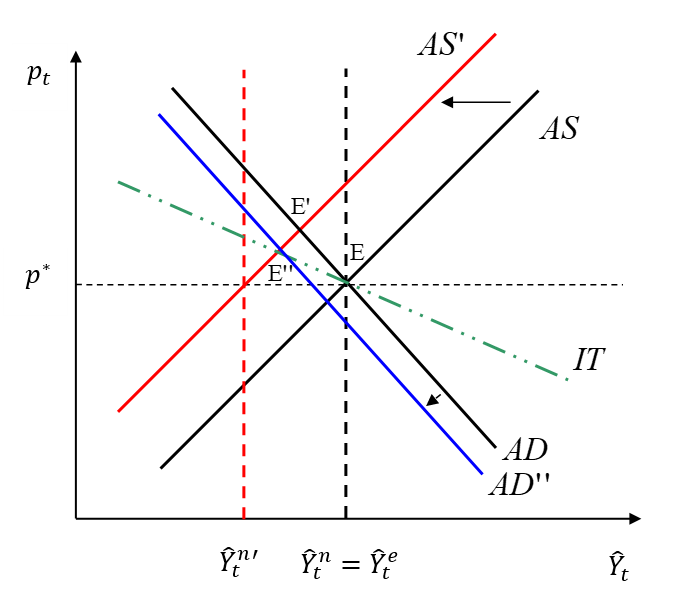
\includegraphics[width=\linewidth]{Figures/Figure9.png}
\end{column}

\end{columns}
\end{frame}

% --- SLIDE 3: Policy Guidance — IT vs. Wicksell ---
\begin{frame}{Policy Guidance: IT vs. Wicksellian Natural Rate}
\small

\textbf{Inflation-Targeting Guidance}
\begin{itemize}
  \item $IT$ gives the welfare‐optimal combination of prices and output.
  \item Policy rate should adjust to shift $AD$ along the $AS$ curve until the economy reaches the locus implyied by $IT$.
\end{itemize}

\vspace{0.25cm}

\textbf{Wicksellian Contrast}
\begin{itemize}
  \item Wicksellian rule follows the frictionless real rate $r_t^{e}$.
  \item $r_t^{e}$ varies only with efficient shocks → unchanged under markup shocks.
  \item Following the guidance of $r_t^{e}$ when there are mark-up shocks delivers a non-optimal allocation.
\end{itemize}

\end{frame}


% ======================================================
\section{Optimal policy under commitment and markup shocks}
\begin{frame}{Optimal Policy: Dynamic Representation}
\small
\begin{itemize}
  \item It is convenient to rewrite the system in terms of the gap between output and its \emph{efficient} level:
\end{itemize}
\begin{equation*}
x_{t}\equiv \hat{Y}_{t}-\hat{Y}_{t}^{e}.
\end{equation*}

\begin{itemize}
  \item \textbf{Rewriting the IS Equation (AD)}
    \begin{equation}
    x_{t}=E_{t}x_{t+1}-\sigma \left( \hat{\imath}_{t}-E_{t}(\pi _{t+1}-\pi)-r_{t}^{e}\right). \label{AD4}
    \end{equation}
  \item \textbf{Rewriting the Phillips Curve (AS)}
    \begin{equation}
    \pi _{t}-\pi =\kappa x_{t}+\upsilon _{t}+\beta E_{t}(\pi _{t+1}-\pi ). \label{AS4}
    \end{equation}
\end{itemize}

\end{frame}

\begin{frame}{Optimal Policy: Dynamic Representation}
\small

\textbf{The Cost-Push Shock ($\upsilon_t$)}
\begin{equation*}
\upsilon _{t}=\kappa (\hat{Y}_{t}^{e}-\hat{Y}_{t}^{n})=\frac{\kappa }{\sigma^{-1}+\eta }\hat{\mu}_{t}.
\end{equation*}

\textbf{The Frictionless Real Rate ($r_t^e$)}
\begin{itemize}
  \item Defined as the rate consistent with flexible prices and efficient output. It summarizes disturbances from productivity, spending, and preferences:
\end{itemize}
\begin{equation*}
r_{t}^{e}\equiv E_{t}\left\{ \frac{1+\eta }{1+\sigma \eta }\left( \hat{A}_{t+1}-\hat{A}_{t}\right) -\frac{\eta }{1+\sigma \eta }(\hat{G}_{t+1}-\hat{G}_{t})-(\hat{\xi}_{t+1}-\hat{\xi}_{t})\right\}.
\end{equation*}

\end{frame}

\begin{frame}{Optimal Policy: Dynamic Representation}
\small

\begin{itemize}
  \item Combining the AS equation \eqref{AS4} with the targeting rule \eqref{InflationTargeting} allows us to eliminate inflation.
  \item This yields a second-order stochastic difference equation for the output gap $x_{t}$:
\end{itemize}

\begin{equation}
E_{t}x_{t+1}-\left( 1+\frac{1}{\beta }+\frac{\kappa \theta }{\beta }\right)
x_{t}+\frac{1}{\beta }x_{t-1}=\frac{\theta }{\beta }\upsilon _{t}.
\label{eqopt}
\end{equation}

\begin{itemize}
  \item The dynamic properties of the optimal allocation depend on the roots of the associated characteristic polynomial $P(\gamma)$:
\end{itemize}

\begin{equation}
P(\gamma )=\gamma ^{2}-\left( 1+\frac{1}{\beta }+\frac{\kappa \theta }{\beta
}\right) \gamma +\frac{1}{\beta }. \label{Poly}
\end{equation}

\end{frame}

\begin{frame}[label=Blanchard]{Optimal Policy: Determinacy and Stability}
\small

\textbf{Conditions for Determinacy (Unique and Stable Solution)}
\begin{itemize}
  \item \textbf{Uniqueness:} Essential for effective policy control. Without uniqueness, multiple equilibrium paths would be consistent with the same policy, undermining the ability to control inflation and output.
  \item \textbf{Stability:} Required for the validity of the log-linear approximation, which is meaningful only for solutions that remain close to the steady state.
\end{itemize}

\vspace{0.2cm}

\textbf{Blanchard--Kahn Conditions}
\begin{itemize}
  \item A linear rational expectations system has a unique and stable solution if the number of eigenvalues inside the unit circle equals the number of predetermined variables.
  \item The difference equation \eqref{eqopt} contains one predetermined variable, $x_{t-1}$.
  \item Therefore, the characteristic polynomial must have exactly \textbf{one eigenvalue inside the unit circle} (stable root) and \textbf{one eigenvalue outside} (unstable root).
\end{itemize}

\vspace{0.3cm}
\begin{center}
\hyperlink{Appendix G}{\beamerbutton{Conditions for Determinacy}}
\end{center}

\end{frame}

\begin{frame}{Determinacy and Stability}
\small

\textbf{Properties of the Polynomial $P(\gamma)$}
\begin{itemize}
  \item We evaluate $P(\gamma)$ at critical points to locate the roots:
\end{itemize}

\begin{equation*}
P(0) = \frac{1}{\beta} > 0, \qquad P(1) = -\frac{\kappa\theta}{\beta} < 0, \qquad P(\infty) = \infty
\end{equation*}



\textbf{Location of Eigenvalues}
\begin{itemize}
  \item Since $P(\gamma)$ is continuous and changes sign between 0 and 1, the first root satisfies $\bm{0 < \gamma_1 < 1}$.
  \item The product of roots is $\gamma_1 \gamma_2 = 1/\beta$. Given $\gamma_1 < 1$ and $\beta < 1$, the second root must satisfy $\bm{\gamma_2 > 1}$.
  \item \textbf{Conclusion:} The eigenvalues satisfy $0 < \gamma_{1} < 1 < \gamma_{2}$. The determinacy condition is met.
\end{itemize}

\end{frame}

\begin{frame}{Solving the Difference Equation: Step 1}
\small

\textbf{Defining the Lag Operator}
\begin{itemize}
    \item Let us define the lag operator ($\mathsf{L}$) with properties $\mathsf{L}\cdot x_{t}=x_{t-1}$ and $\mathsf{L}^{-1}\cdot x_{t}=E_{t}x_{t+1}$.
    \item More generally, $\mathsf{L}^{k}\cdot x_{t}=x_{t-k}$ and $\mathsf{L}^{-k}\cdot x_{t}=E_{t}x_{t+k}$.
\end{itemize}

\textbf{Rewriting the Equation}
\begin{itemize}
    \item We can then write equation (\ref{eqopt}) as:
\end{itemize}
\begin{equation*}
\left[ \mathsf{L}^{-1}-\left( 1+\frac{1}{\beta }+\frac{\kappa \theta }{\beta
}\right) +\frac{1}{\beta }\mathsf{L}\right] x_{t}=\frac{\theta }{\beta }%
\upsilon _{t}.
\end{equation*}

\textbf{Substituting Roots}
\begin{itemize}
\item Note that $\gamma_1+\gamma_2=\left( 1+\frac{1}{\beta }+\frac{\kappa \theta }{\beta
}\right)$ and $\gamma_1\gamma_2=\frac{1}{\beta }.$
    \item Therefore, using the sum and product of roots:
\end{itemize}
\begin{equation*}
\left[ \mathsf{L}^{-1}-\left( \gamma _{1}+\gamma _{2}\right) +\gamma
_{1}\gamma _{2}\mathsf{L}\right] x_{t}=\theta \gamma _{1}\gamma _{2}\upsilon
_{t}.
\end{equation*}

\end{frame}

\begin{frame}{Solving the Difference Equation: Step 2}
\small

\textbf{Factorization}
\begin{itemize}
    \item We can factor the previous expression into stable and unstable components:
\end{itemize}
\begin{equation*}
(1-\gamma _{1}\mathsf{L})(\mathsf{L}^{-1}-\gamma _{2})x_{t}=\theta \gamma
_{1}\gamma _{2}\upsilon _{t}.
\end{equation*}

\textbf{Simplification}
\begin{itemize}
    \item We can further simplify the above expression to:
\end{itemize}
\begin{equation*}
(1-\gamma _{1}\mathsf{L})(1-\gamma _{2}^{-1}\mathsf{L}^{-1})x_{t}=-\theta
\gamma _{1}\upsilon _{t}.
\end{equation*}

\textbf{Forward solution for the unstable block}
\begin{itemize}
    \item It follows that:
\end{itemize}
\begin{eqnarray}
(1-\gamma _{1}\mathsf{L})x_{t} &=&-\frac{\theta \gamma _{1}}{(1-\gamma
_{2}^{-1}\mathsf{L}^{-1})}\upsilon _{t} \notag \\
&=&-\theta \gamma _{1}E_{t}\sum_{j=0}^{\infty }\gamma _{2}^{-j}\upsilon
_{t+j}. \label{Sol33}
\end{eqnarray}

\end{frame}

\begin{frame}{Mathematical Tool: Geometric Series}
\small

\begin{itemize}
    \item In going from the first to the second line of the previous slide, we noticed that:
\end{itemize}
\begin{eqnarray*}
\frac{\upsilon _{t}}{1-\gamma _{2}^{-1}\mathsf{L}^{-1}} &=&(1+\gamma
_{2}^{-1}\mathsf{L}^{-1}+\gamma _{2}^{-2}\mathsf{L}^{-2}+\gamma _{2}^{-3}%
\mathsf{L}^{-3}+...)\upsilon _{t} \\
&=&E_{t}\sum_{j=0}^{\infty }\gamma _{2}^{-j}\upsilon _{t+j}.
\end{eqnarray*}
\begin{itemize}
    \item We used the properties of the operator $\mathsf{L}^{-k}$ for $k\geq 1.$
\end{itemize}
\begin{itemize}
    \item To remember the above expansion, recall that for a generic real number $c$ with $|c|<1$:
    \begin{equation*}
    \frac{1}{1-c}=\sum_{j=0}^{\infty }c^{j}.
    \end{equation*}
    \item Set $c=\gamma _{2}^{-1}\mathsf{L}^{-1}$ and note that $\gamma _{2}>1$, therefore the result follows.
\end{itemize}

\end{frame}

\begin{frame}{Dynamic Solution: The Output Gap}
\small

\begin{itemize}
    \item Using $\mathsf{L}x_{t}=x_{t-1}$, we can write \eqref{Sol33} as:
\end{itemize}
\begin{equation*}
x_{t}=\gamma _{1}x_{t-1}-\theta \gamma _{1}E_{t}\sum_{j=0}^{\infty }\gamma
_{2}^{-j}\upsilon _{t+j}.
\end{equation*}

\textbf{White Noise Assumption}
\begin{itemize}
    \item For the sake of simplicity, let us assume that $\upsilon _{t}$ is a white-noise shock, therefore $E_{t}\upsilon _{t+j}=0$ for each $j>0$ and then:
\end{itemize}
\begin{equation*}
x_{t}=\gamma _{1}x_{t-1}-\theta \gamma _{1}\upsilon _{t}.
\end{equation*}

\textbf{Interpretation}
\begin{itemize}
    \item The above equation represents the dynamic solution for output gap, showing that it falls on impact when mark-up increases.
\end{itemize}

\end{frame}

\begin{frame}{Dynamic Solution: Inflation and Interest Rates}
\small

\textbf{Path of Inflation}
\begin{itemize}
    \item The path of inflation follows from (\ref{InflationTargeting}) and is represented by:
\end{itemize}
\begin{equation*}
(\pi _{t}-\pi )=-\theta ^{-1}(\gamma _{1}-1)x_{t-1}+\gamma _{1}\upsilon _{t}.
\end{equation*}
\begin{itemize}
    \item Inflation rises above target at the time in which the markup shock hits.
\end{itemize}

\textbf{Path of Interest Rate}
\begin{itemize}
    \item Using the AD equation \eqref{AD4}, we derive the path consistent with optimal policy:
\end{itemize}
\begin{eqnarray}
\hat{\imath}_{t} &=&r_{t}^{e}+E_{t}(\pi _{t+1}-\pi )+\sigma
^{-1}E_{t}(x_{t+1}-x_{t}) \notag \\
\hat{\imath}_{t} &=&r_{t}^{e}-(\sigma ^{-1}-\theta ^{-1})(1-\gamma
_{1})x_{t} \label{iopt2}
\end{eqnarray}
\begin{itemize}
    \item This shows the nominal interest rate should follow the frictionless real rate and react inversely to the output gap (provided $\sigma<\theta$).
\end{itemize}

\end{frame}
\begin{frame}{Interpretation of the Interest Rate Path}
\small

\textbf{Not an Instrument Rule}
\begin{itemize}
    \item Equation (\ref{iopt2}) should \textbf{not} be interpreted as the interest rate rule the policymaker follows to implement optimal policy.
    \item Instead, it represents the \textit{resulting path} of the policy rate once the central bank achieves the targeting rule (\ref{InflationTargeting}).
    \item \textbf{Note:} If (\ref{iopt2}) were used as a mechanical instrument rule, it would lead to \textbf{equilibrium indeterminacy}.
\end{itemize}

\textbf{The Role of R-star ($r^*$)}
\begin{itemize}
    \item The equation shows that matching the Wicksellian real rate is a useful check when responding to \textbf{efficient shocks}.
    \item However, this does \textbf{not} hold when dealing with \textbf{inefficient disturbances}.
    \item \textbf{Policy Implication:} Strategies focusing on R-star (frictionless rate) must be cautious, as simple tracking is insufficient during inefficient shocks.
\end{itemize}

\end{frame}

\begin{frame}{Optimal Policy with Commitment}
\small

\textbf{Inertia and Expectations}
\begin{itemize}
    \item Under optimal policy with commitment, inflation and the output gap show \textbf{inertial behavior}, since the AS equation (\ref{AS4}) depends on expectations ($E_t \pi_{t+1}$). Managing these expectations is critical for maximum welfare.
\end{itemize}

\textbf{Dynamic Response to a Markup Shock}
\begin{itemize}
    \item \textbf{Inflation:} Rises above target on impact, but then falls \textit{below} target to meet it in the long run.
    \item \textbf{Prices:} Rise initially (more than target requires), but subsequently their growth rate falls below the target rate.
    \item \textbf{Interest Rate:} Inherits the persistent behavior of the output gap. Even if the shock lasts only one period, the rate remains above steady state for a long time, declining only gradually.
\end{itemize}
\end{frame}


% ======================================================
% ======================================================
\section{Optimal Policy under Discretion\label{Chapter7-D}}

\begin{frame}{Optimal Policy Under Discretion}
\small

\begin{itemize}
    \item \textbf{Re-optimization:} Discretion implies the policymaker re-optimizes each period; past promises are not honored.
    \item \textbf{Expectations:} Private agents internalize this. They form expectations knowing the policymaker will not commit to future actions.
    \item The forward-looking AS equation links current outcomes to expected future policy, causing discretion to yield a different inflation–output path than commitment.
    \item With discretion and linear-quadratic optimization problem, equilibrium allocations must be linear functions of the economy’s state variables.
    \item In this setting, the only state variable is the markup shock $\upsilon_t$ (assumed white noise).
\end{itemize}

\end{frame}

\begin{frame}{Constructing the Discretionary Equilibrium}
\small

\textbf{Guessed Functional Form}
\begin{itemize}
    \item Since $\upsilon_t$ is the only state variable, we guess a linear solution of the form:
\end{itemize}

\begin{equation*}
(\pi_t - \pi) = \pi_d \upsilon_t, \qquad x_t = x_d \upsilon_t
\end{equation*}

\textbf{Implication for Expectations}
\begin{itemize}
    \item Because $\upsilon_t$ is white noise ($E_t \upsilon_{t+1} = 0$), inflation expectations are zero:
\end{itemize}

\begin{equation*}
E_t(\pi_{t+1}-\pi) = E_t(\pi_d \upsilon_{t+1}) = 0
\end{equation*}

\end{frame}

\begin{frame}{Optimization Problem Under Discretion}
\small

\textbf{Objective}
\begin{itemize}
    \item Only the current-period loss matters, since inflation and output depend solely on the current shock $\upsilon_t$.
\end{itemize}

\begin{equation*}
\min_{\pi_d, x_d} \quad \frac{1}{2} (x_d \upsilon_t)^2 + \frac{1}{2} \frac{\theta}{\kappa} (\pi_d \upsilon_t)^2
\end{equation*}

\textbf{AS Constraint}
\begin{itemize}
    \item We substitute the guess and the expectation into the AS equation (\ref{AS4}). This yields a static constraint on the coefficients:
\end{itemize}

\begin{equation*}
\pi_d \upsilon_t = \kappa x_d \upsilon_t + \upsilon_t
\end{equation*}

\end{frame}

\begin{frame}{Optimal Solution and Targeting Rule}
\small

\textbf{Optimal Coefficients}
\begin{itemize}
    \item Solving the minimization problem subject to the constraint yields the optimal responses to the shock:
\end{itemize}

\begin{equation*}
x_{d}=-\frac{\theta }{1+\theta \kappa }, \qquad \pi _{d}=\frac{1}{1+\theta \kappa }.
\end{equation*}


\begin{itemize}
    \item Combining these expressions implies a linear relationship between inflation and the output gap:
\end{itemize}
\textbf{The Discretionary Targeting Rule}
\begin{equation}
(\pi _{t}-\pi )+\theta ^{-1}x_t = 0.
\label{IT2}
\end{equation}


\end{frame}

\begin{frame}{Comparison: Discretion vs. Commitment}
\small

\textbf{Lack of Inertia}
\begin{itemize}
    \item Differently from commitment, optimal policy under discretion \textbf{does not feature any inertia}.
    \item It implies a different short-run response to the shock.
\end{itemize}

\begin{itemize}
    \item Comparing the targeting rules:
    \begin{itemize}
        \item \textbf{Discretion (\ref{IT2}):} Trade-off between inflation and the \textbf{level} of the output gap.
        \item \textbf{Commitment (\ref{InflationTargeting}):} Trade-off involves the \textbf{growth rate} of the output gap ($x_t - x_{t-1}$).
    \end{itemize}
    \item Under commitment, the policymaker cares about output growth (internalizing past levels). This reflects the necessity of fulfilling past promises, resulting in a inertial plan.
\end{itemize}
\end{frame}

\begin{frame}{Interest Rate Rules}
\small

\begin{itemize}
\item We now move away from the "optimal policy" derived previously.
    \item Instead, we assume the policymaker follows a specific \textbf{interest-rate rule} (often called a Taylor-type rule): 
\end{itemize}

\begin{equation} \label{IRR}
\hat{\imath}_{t}
=
r_{t}^{e}
+
\phi_{\pi}(\pi_t-\pi)
+
\phi_{x}x_t.
\end{equation}

\begin{itemize}
    \item The rule incorporates a one-to-one response to the frictionless real rate, taken as perfectly predictable to isolate inefficient (markup) shocks. 
    \item \textbf{Note}: original Taylor rule does not consider a response to the frictionless real rate.
  
\end{itemize}

\end{frame}



\begin{frame}{Policy Reaction Parameters}
\small

\textbf{Structure of the Rule}
\begin{itemize}
    \item Two reaction components govern policy:
    \begin{itemize}
        \item Inflation deviation: \(\phi_\pi(\pi_t-\pi)\)
        \item Output gap: \(\phi_x x_t\)
    \end{itemize}
    \item Parameters satisfy \(\phi_\pi \ge 0\), \(\phi_x \ge 0\).
\end{itemize}

\textbf{Interpretation}
\begin{itemize}
    \item \(\phi_\pi\): weight placed on inflation stability.
    \item \(\phi_x\): weight placed on output-gap stabilization.
    \item Choice of parameters encodes the central bank’s preference mix under interest rule-based policy.
\end{itemize}

\end{frame}

\begin{frame}{Model Under an Interest Rate Rule}
\small

\textbf{System Reduction}
\begin{itemize}
    \item Adding (\ref{IRR}) to (\ref{AD4}) and (\ref{AS4}) initially gives three equations for three variables ($\hat{\imath}_{t}$, $\pi _{t}$, $x_{t}$).
    \item We use (\ref{AS4}) and (\ref{IRR}) into (\ref{AD4}) to substitute for $\hat{\imath}_{t}$ and $E_{t}(\pi _{t+1}-\pi )$.
    \item This compresses the model into a system of two stochastic linear difference equations:
\end{itemize}

\begin{equation}
E_{t}\begin{bmatrix}
\pi _{t+1}-\pi \\
x_{t+1}
\end{bmatrix}
=
\begin{bmatrix}
\frac{1}{\beta } & -\frac{\kappa }{\beta } \\
\sigma (\phi _{\pi }-\frac{1}{\beta }) & 1+\sigma \phi _{x}+\sigma \frac{\kappa }{\beta }
\end{bmatrix}
\begin{bmatrix}
\pi _{t}-\pi \\
x_{t}
\end{bmatrix}
+
\begin{bmatrix}
-\frac{1}{\beta } \\
\frac{\sigma }{\beta }
\end{bmatrix}
\upsilon _{t}
\label{System}
\end{equation}

\textbf{Implication}
\begin{itemize}
    \item Because the rule offsets movements in the frictionless real rate, dynamics of inflation and the output gap depend solely on the markup disturbance.
\end{itemize}

\end{frame}

\begin{frame}{Determinacy and Stability Analysis}
\small

\textbf{1. Blanchard-Kahn Conditions}
\begin{itemize}
    \item \textbf{Rule:} The number of eigenvalues within the unit circle must equal the number of predetermined variables.
    \item \textbf{Application:} In system (\ref{System}), there are \textbf{no predetermined variables} (no terms indexed $t-1$).
    \item \textbf{Requirement:} For a unique, bounded solution, both eigenvalues must lie outside the unit circle ($|\gamma| > 1$).
\end{itemize}
\end{frame}
\begin{frame}{Matrix $\mathcal{V}$}
\small
    \textbf{2. The Characteristic Polynomial}
\begin{itemize}
    \item Consider the matrix $\mathcal{V}$ from system (\ref{System}):
    \begin{equation*}
    \mathcal{V}=\begin{bmatrix}
    \frac{1}{\beta } & -\frac{\kappa }{\beta } \\
    \sigma (\phi _{\pi }-\frac{1}{\beta }) & 1+\sigma \phi _{x}+\sigma \frac{\kappa }{\beta }
    \end{bmatrix}
    \end{equation*}
    \item The characteristic polynomial is given by $P(\gamma )=\gamma ^{2}-tr[\mathcal{V}]\gamma +\det [\mathcal{V}]$.
    \item Trace and determinant are both positive:
    \begin{eqnarray*}
    tr[\mathcal{V}] &=&\left( 1+\frac{1}{\beta }+\sigma \phi _{x}+\sigma \frac{\kappa }{\beta }\right) >0 \\
    \det [\mathcal{V}] &=&\frac{1}{\beta }\left( 1+\sigma \phi _{x}+\sigma \kappa \phi _{\pi }\right) >0
    \end{eqnarray*}
\end{itemize}
\end{frame}

\begin{frame}{Determinacy under Interest Rate Rules}
\small

\textbf{Location of the Eigenvalues}
\begin{itemize}
    \item Since $tr[\mathcal{V}] > 0$ and $\det[\mathcal{V}] > 0$, both eigenvalues of the system matrix $\mathcal{V}$ are positive.
    
    \item To determine whether the roots lie inside or outside the unit circle, we evaluate the characteristic polynomial $P(\gamma)$ at key points:
    \begin{itemize}
        \item $P(0) = \det[\mathcal{V}] > 0$
        \item $P(\infty) = \infty$
    \end{itemize}

    \item \textbf{Determinacy condition:} For both eigenvalues to lie outside the unit circle (no predetermined variables), we require:
    \begin{equation}
    P(1)
    = \sigma \phi_x(\beta^{-1}-1)
    + \sigma \kappa \beta^{-1}(\phi_\pi - 1)
    > 0.
    \label{TaylorPrinciple}
    \end{equation}
\end{itemize}

\end{frame}

\begin{frame}{The Taylor Principle}
\small

\textbf{The Taylor Principle}
\begin{itemize}
    \item Condition \eqref{TaylorPrinciple} is known as the \textbf{generalized Taylor principle}.
    \item It ensures a \textbf{unique and stable equilibrium} by preventing self-fulfilling fluctuations driven by expectations.
\end{itemize}

\vspace{0.1cm}

\textbf{Special Case}
\begin{itemize}
    \item If the policy rule does not respond to the output gap ($\phi_x = 0$), the condition simplifies to:
    \[
    \phi_\pi > 1.
    \]
    \item This is the classic \textbf{Taylor principle}.
\end{itemize}

\vspace{0.1cm}

\textbf{Economic Intuition}
\begin{itemize}
    \item A one-percent increase in inflation must trigger a \emph{more than one-percent} increase in the nominal interest rate.
    \item This raises the \textbf{real interest rate}, dampening aggregate demand and stabilizing inflation.
    \item If $\phi_\pi \le 1$, higher expected inflation lowers the real rate, leading to \textbf{self-fulfilling inflation dynamics} and equilibrium indeterminacy.
\end{itemize}

\end{frame}


\begin{frame}{Characterizing the Unique Solution}
\small

\textbf{Prerequisites}
\begin{itemize}
    \item Under condition (\ref{TaylorPrinciple}), we can now characterize the unique and stable solution.
    \item \textbf{Assumption:} For simplicity, let us assume again that $\upsilon _{t}$ follows a white-noise process.
\end{itemize}

\textbf{Method of Undetermined Coefficients}
\begin{itemize}
    \item One way to characterize the solution is to guess that the equilibrium variables are linear functions of the shock $\upsilon _{t}$.
    \item We posit the following form:
\end{itemize}

\begin{equation*}
\pi _{t}-\pi =\pi _{r}\upsilon _{t},
\end{equation*}
\begin{equation*}
x_{t}=x_{r}\upsilon _{t}.
\end{equation*}
\end{frame}

\begin{frame}{Deriving the Parameter Restrictions}
\small

\begin{itemize}
    \item Inserting the hypothesized solution into the first line of system (\ref{System}):
    \begin{equation*}
    \pi _{r}E_{t}\upsilon _{t+1}=\frac{1}{\beta }\pi _{r}\upsilon _{t}-\frac{%
    \kappa }{\beta }x_{r}\upsilon _{t}-\frac{1}{\beta }\upsilon _{t}.
    \end{equation*}
    \item Since $E_{t}\upsilon _{t+1}=0$ (white noise), we simplify to obtain the first restriction between unknown parameters:
\end{itemize}
\begin{equation}
\pi _{r}=\kappa x_{r}+1. \label{sol1}
\end{equation}

\begin{itemize}
    \item From the second line of (\ref{System}), we obtain:
    \begin{equation*}
    x_{r}E_{t}\upsilon _{t+1}=\sigma \left( \phi _{\pi }-\frac{1}{\beta }\right)
    \pi _{r}\upsilon _{t}+\left( 1+\sigma \phi _{x}+\sigma \frac{\kappa }{\beta }%
    \right) x_{r}\upsilon _{t}+\frac{\sigma }{\beta }\upsilon _{t}.
    \end{equation*}
    \item Setting the LHS to zero and rearranging yields the second restriction:
\end{itemize}
\begin{equation}
\left( \frac{1}{\beta }-\phi _{\pi }\right) \pi _{r}=\left( \sigma
^{-1}+\phi _{x}+\frac{\kappa }{\beta }\right) x_{r}+\frac{1}{\beta }.
\label{sol2}
\end{equation}

\end{frame}

\begin{frame}{Solution and Policy Trade-offs}
\small

\begin{itemize}
    \item Combining the restrictions (\ref{sol1}) and (\ref{sol2}), we obtain the final coefficients:
\end{itemize}
\begin{equation*}
x_{r}=-\frac{\phi _{\pi }}{\sigma ^{-1}+\phi _{x}+\kappa \phi _{\pi }}, \qquad
\pi _{r}=\frac{\sigma ^{-1}+\phi _{x}}{\sigma ^{-1}+\phi _{x}+\kappa \phi _{\pi }}
\end{equation*}

\textbf{General Dynamics}
\begin{itemize}
    \item The parameters satisfy $\pi _{r}\geq 0$ and $x_{r}\leq 0$.
    \item A markup shock puts upward pressure on inflation and reduces the output gap (relative to the efficient level).
\end{itemize}
\end{frame}
\begin{frame}{Limiting cases under Interest Rate Rule}
\small

Varying policy parameters $\phi _{\pi }$ and $\phi _{x}$ reveals the trade-off along the structural constraint $\pi _{r}=\kappa x_{r}+1$.

\vspace{0.3cm}

\begin{columns}[t]

% LEFT COLUMN
\begin{column}{0.48\textwidth}
\textbf{Strict Inflation Targeting ($\phi _{\pi }\rightarrow \infty $)}
\begin{itemize}
\item \textbf{Result:} $\pi _{r} \to 0$ and $x_{r} \to -1/\kappa$.
\item Inflation is perfectly stabilized.
\item The entire shock is absorbed by a sharp fall in output.
\end{itemize}
\end{column}

% RIGHT COLUMN
\begin{column}{0.48\textwidth}
\textbf{Strict Output Targeting ($\phi _{x}\rightarrow \infty $)}
\begin{itemize}
\item \textbf{Result:} $x_{r} \to 0$ and $\pi _{r} \to 1$.
\item Output is perfectly stabilized.
\item There is full pass-through of the markup shock into inflation.
\end{itemize}
\end{column}

\end{columns}

\end{frame}

\begin{frame}{Dynamic Responses after a Markup Shock}
\small

\begin{columns}
\begin{column}{0.55\textwidth}
{
\setbeamertemplate{caption}{\raggedright\insertcaption\par}
\begin{figure}
\centering
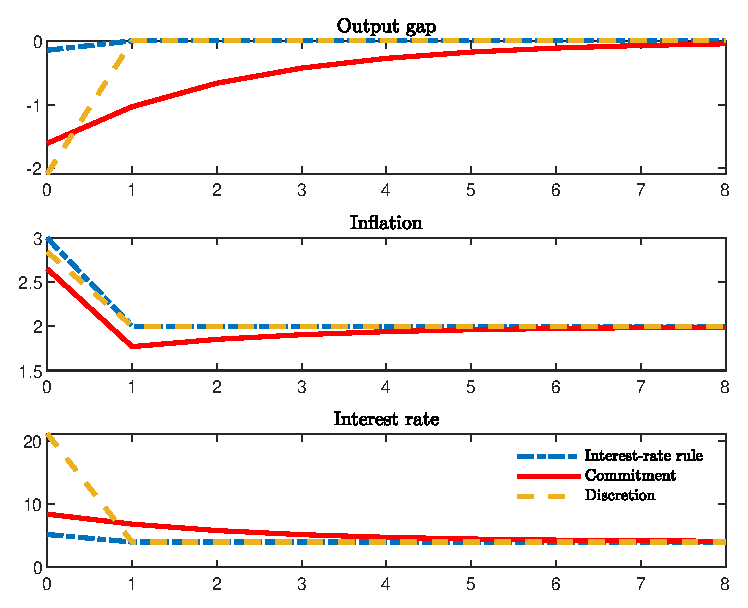
\includegraphics[width=0.9\linewidth]{Figures/Figure10.eps}
\caption{\tiny Note: The Figure uses the following parametrization: $\beta =0.995,$ $%
\kappa =0.02,$ $\sigma =0.5,$ $\theta =10,$ $\eta =0.47$, $\phi _{y}=0.5$, $%
\phi _{\pi }=1.5.$ The one-period markup shock ($\upsilon $) is set at
0.25\%. The model is calibrated quarterly. Inflation target $\pi $ is set at
a 2\% annual rate. Output gap in \%, inflation and interest rate in annualized \%.}
\end{figure}
}
\end{column}


\begin{column}{0.45\textwidth}
    \textbf{Comparison of Policies}
    \begin{itemize}
        \item We compare the impulse responses of the output gap, inflation, and interest rate after a positive temporary markup shock ($\upsilon = 0.25\%$) under commitment, discretion, and an interest-rate rule. 
        \item \textbf{Commitment:} Variables display a \textbf{inertial response}, despite the shock lasting only one period.
        \item \textbf{Discretion \& Rule:} The response dies out immediately as the shock reverts to zero.
    \end{itemize}
\end{column}
\end{columns}
\end{frame}

\begin{frame}{Dynamic Response of the Price Level}
\small

\begin{columns}
\begin{column}{0.55\textwidth}
{
\setbeamertemplate{caption}{\raggedright\insertcaption\par}
\begin{figure}
\centering
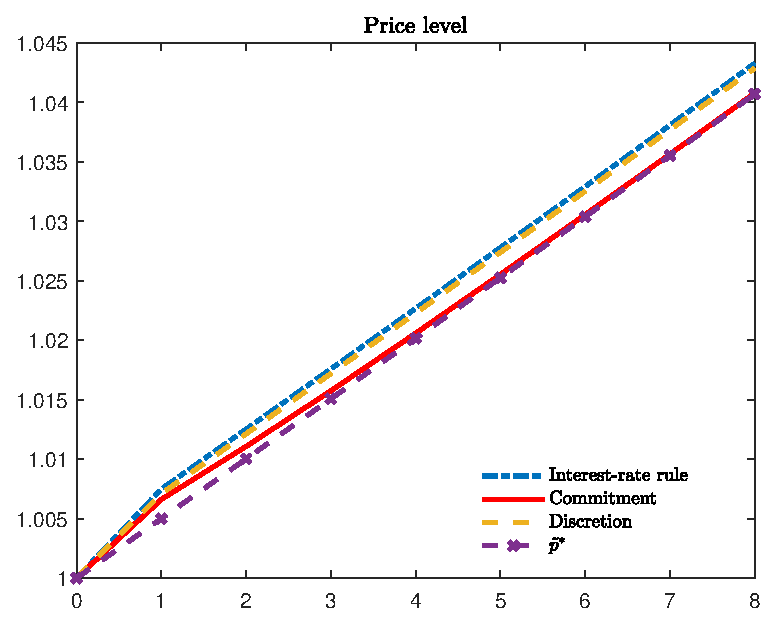
\includegraphics[width=1\linewidth]{Figures/Figure11.eps}
\caption{\tiny Note: Price path following the shock. The line $\tilde{p}^{\ast}$ represents the 2\% trend.}
\end{figure}
}
\end{column}


\begin{column}{0.45\textwidth}
    \textbf{Comparison of Policies}
    \begin{itemize}
        \item \textbf{Commitment:} The initial rise in prices is \textbf{undone} in subsequent periods. The price level returns to the pre-shock trend ($\tilde{p}^{\ast }$).
        \item \textbf{Discretion \& Rule:} Prices jump and then grow at the 2\% rate from the \textit{new, higher} level. They never reconnect to the initial trend.
    \end{itemize}
    \textbf{Conclusion}
    \begin{itemize}
        \item Under discretion, "bygones are bygones."
        \item Commitment maintains long-term price stability.
    \end{itemize}
\end{column}
\end{columns}
\end{frame}

\section{Optimal Inflation Target\label{Chapter7-IT}}
\begin{frame}{Why a Positive Inflation Target? ($\pi > 0$)}
\small

Three main reasons justify a positive inflation target:

\vspace{0.4cm}

\begin{enumerate}
    \item \textbf{ZLB Buffer:} A higher inflation target implies a higher steady-state nominal interest rate.
    This provides a safety margin for the central bank to offset negative shocks to the \emph{frictionless real rate} $\hat{r}_t^{e}$ before the zero lower bound ($i_t \ge 0$) becomes binding.
    
    \vspace{0.2cm}
    
    \item \textbf{Downward Wage Rigidity:} Nominal wages are rigid downward.
    Positive inflation acts as “grease” in the labor market (\cite{tobin1972}), allowing real wages to adjust downward without nominal wage cuts, thereby reducing employment and output volatility.
    
    \vspace{0.2cm}
    
    \item \textbf{Debt–Deflation Risk:} With $\pi = 0$, adverse shocks may trigger deflation, increasing the real burden of nominal debt (\cite{fisher1933}).
    This can induce a self-reinforcing contraction in demand, output, and prices.
\end{enumerate}

\end{frame}

\begin{frame}{Quantitative Targets: Research Findings}
\small

While qualitative arguments support $\pi > 0$, quantitative research narrows the optimal range based on specific structural features:

\vspace{0.3cm}

\begin{itemize}
    \item \textbf{ZLB and Indexing:} Accounting for ZLB costs suggests $\pi^* \approx 2\%$ (\cite{coibion2012}). Note: If firms do not index to a target, costs of $\pi > 0$ rise, potentially underestimating the optimal rate.
    
    \vspace{0.2cm}
    
    \item \textbf{Endogenous Entry:} In models with product variety and firm entry, deviations from long-run price stability are optimal (\cite{bilbie2014}).
    
    \vspace{0.2cm}
    
    \item \textbf{Productivity Trends:} In frameworks with heterogeneous productivity trends across firms, the optimal rate is estimated between 1\% and 3\% (\cite{adam2019}).
    
    \vspace{0.2cm}
    
    \item \textbf{Measurement Bias:} A positive target acknowledges quality improvements and new goods not previously captured in standard price indices.
\end{itemize}

\end{frame}

\begin{frame}{The Upper Bound: Costs of High Inflation}
\small

Why not target much higher inflation? Significant distortions arise as $\pi$ increases:

\vspace{0.3cm}

\begin{itemize}
    \item \textbf{Tax Distortions:} Interaction with non-indexed tax brackets increases effective tax rates and distorts incentives (\cite{feldstein1997}).
    
    \vspace{0.2cm}
    
    \item \textbf{Information and Signal Noise:} High inflation obscures relative price signals and complicates long-term planning for investment and credit.
    
    \vspace{0.2cm}
    
    \item \textbf{Volatility and Misallocation:} High $\pi$ is empirically associated with higher inflation volatility (\cite{imf2015}), leading to resource misallocation.
    
    \vspace{0.2cm}
    
    \item \textbf{Expectations De-anchoring:} High, volatile inflation increases the "attention" agents pay to prices, making expectations more volatile and harder to control.
\end{itemize}

\vspace{0.3cm}
\textbf{Conclusion:} Current targets (1\%--3\%) represent a reasonable balance between avoiding the ZLB and minimizing distortionary costs.

\end{frame}

% ======================================================
\section{Main Takeaways}
\begin{frame}{Main Takeaways}
\small
\begin{itemize}
  \item \textbf{Flexible Inflation Targeting}: optimal under commitment; allows temporary inflation deviations only in exchange for deviations of \textbf{output growth from the efficient growth trend}.
  \item \textbf{Optimal Targeting Rule}:
  \[
  (\pi_t - \pi) + \theta^{-1}(\Delta \hat{Y}_t - \Delta \hat{Y}_t^e) = 0.
  \]
  \item \textbf{History Dependence}: commitment is equivalent to \textbf{price-level targeting}; it implies \textbf{price-level reversion} after inefficient shocks.
  \item \textbf{Discretion}: sub-optimal because it trades off inflation with the \emph{level} of the output gap and lacks inertia (expectations management).
  \item \textbf{Taylor Rule}: determinacy requires a generalized Taylor principle; when $\phi_x=0$ it reduces to $\phi_\pi>1$.
  \item \textbf{The Numerical Target}: structural frictions (ZLB, wage rigidity, debt-deflation) justify a positive $\pi$ and support targets in the \textbf{1--3\% range}.
\end{itemize}
\end{frame}


\appendix
\section{Appendix: Derivations}
\begin{frame}[label=Appendix F]{Derivation of equation \eqref{LossNK}}
\small
Consider the expected utility of the consumers (5.1) and write
it as%
\begin{equation*}
U_{t_{0}}=E_{t_{0}}\left\{ \sum_{t=t_{0}}^{+\infty }\beta ^{t-t_{0}}\xi _{t} 
\left[ \left( U(C_{t})-H(L_{t})\Delta _{t}\right) \right] \right\} ,
\end{equation*}%
\begin{equation*}
U(C_{t})=\frac{C_{t}^{1-\frac{1}{\tilde{\sigma}}}}{1-\frac{1}{\tilde{\sigma}}%
}
\end{equation*}%
\begin{equation*}
H(L_{t})=\frac{L_{t}^{1+\eta }}{1+\eta },
\end{equation*}% 
\begin{equation*}
\Delta _{t}\equiv \int_{0}^{1}\left( \frac{p_{t}(j)}{P_{t}}\right) ^{-\theta
(1+\eta )}dj.
\end{equation*}%
Observe, indeed, that 
\begin{equation*}
L_{t}(j)=\frac{Y_{t}(j)}{A_{t}}=\left( \frac{p_{t}(j)}{P_{t}}\right)
^{-\theta }\frac{Y_{t}}{A_{t}}=\left( \frac{p_{t}(j)}{P_{t}}\right)
^{-\theta }L_{t}.
\end{equation*}%
\end{frame}

\begin{frame}\small
Note the following second-order Taylor approximation%
\begin{eqnarray}
\frac{C_{t}^{1-\frac{1}{\tilde{\sigma}}}}{1-\frac{1}{\tilde{\sigma}}} &=&%
\frac{C^{1-\frac{1}{\tilde{\sigma}}}}{1-\frac{1}{\tilde{\sigma}}}+C^{-\frac{1%
}{\tilde{\sigma}}}(C_{t}-C)-\frac{1}{2}\frac{1}{\tilde{\sigma}}C^{-\frac{1}{%
\tilde{\sigma}}-1}(C_{t}-C)^{2}+\mathcal{O}(||\xi ||^{3})  \notag \\
&=&\frac{C^{1-\frac{1}{\tilde{\sigma}}}}{1-\frac{1}{\tilde{\sigma}}}+C^{1-%
\frac{1}{\tilde{\sigma}}}\hat{C}_{t}+\frac{1}{2}\left( 1-\frac{1}{\tilde{%
\sigma}}\right) C^{1-\frac{1}{\tilde{\sigma}}}\hat{C}_{t}{}^{2}+\mathcal{O}%
(||\xi ||^{3})  \label{Capprox}
\end{eqnarray}%
where $\mathcal{O}(||\xi ||^{3})$ collects terms of order higher than the
second and where, in the second line, we have used the following
approximation:%
\begin{equation*}
\left( \frac{C_{t}-C}{C}\right) =\hat{C}_{t}+\frac{1}{2}\hat{C}_{t}^{2}+%
\mathcal{O}(||\xi ||^{3}).
\end{equation*}%
\end{frame}
\begin{frame}\small
Similarly, we can write%
\begin{eqnarray}
H(L_{t})\Delta _{t} &=&H(L)+H_{l}(L_{t}-L)+\frac{1}{2}H_{ll}(L_{t}-L)^{2}+ 
\notag \\
&&+H(L)(\Delta _{t}-1)+\mathcal{O}(||\xi ||^{3})  \notag \\
&=&H(L)+H_{l}L\hat{L}_{t}+\frac{1}{2}H_{l}L\left( 1+\eta \right) \hat{L}%
_{t}^{2}+  \notag \\
&&+H(L)(\Delta _{t}-1)+\mathcal{O}(||\xi ||^{3}),  \label{Happrox}
\end{eqnarray}%
having used $\eta =H_{ll}Y/H_{l}$ and the fact that the expansion of $\Delta
_{t}$ is of second-order magnitude, as it will be shown.

Combining (\ref{Capprox}) and (\ref{Happrox}), we obtain%
\begin{eqnarray}
U(C_{t})-H(L_{t})\Delta _{t} &=&U(C)-H(L)\Delta +U_{c}\hat{C}_{t}+\frac{1}{2}%
U_{c}C\left( 1-\frac{1}{\tilde{\sigma}}\right) \hat{C}_{t}^{2}-H_{l}L\hat{L}%
_{t}+  \notag \\
&&-\frac{1}{2}H_{l}L\left( 1+\eta \right) \hat{L}_{t}^{2}-H(Y)(\Delta
_{t}-1)+\mathcal{O}(||\xi ||^{3}).  \label{Uapprox2}
\end{eqnarray}%
\end{frame}

\begin{frame}\small
Note that, given $Y_{t}=A_{t}L_{t},$ it holds exactly that%
\begin{equation}
\hat{L}_{t}=\hat{Y}_{t}-\hat{A}_{t},  \label{Lapp}
\end{equation}%
whereas a second-order expansion of the equilibrium in the goods market $%
Y_{t}=C_{t}+G_{t}$ implies%
\begin{equation*}
Y_{t}-Y=C_{t}-C+G_{t}-G
\end{equation*}%
and therefore

\begin{equation*}
\hat{Y}_{t}+\frac{1}{2}\hat{Y}_{t}^{2}=\frac{C}{Y}\left( \hat{C}_{t}+\frac{1%
}{2}\hat{C}_{t}^{2}\right) +\hat{G}_{t}+\mathcal{O}(||\xi ||^{3})
\end{equation*}%
using definition $\hat{G}_{t}=(G_{t}-G)/Y.$ We can then write%
\begin{equation*}
\hat{C}_{t}=\frac{Y}{C}\left( \hat{Y}_{t}-\hat{G}_{t}\right) +\frac{1}{2}%
\frac{Y}{C}\hat{Y}_{t}^{2}-\frac{1}{2}\hat{C}_{t}^{2}+\mathcal{O}(||\xi
||^{3})
\end{equation*}%
and therefore%
\begin{equation}
\hat{C}_{t}=\frac{Y}{C}\left( \hat{Y}_{t}-\hat{G}_{t}\right) +\frac{1}{2}%
\frac{Y}{C}\hat{Y}_{t}^{2}-\frac{1}{2}\frac{Y^{2}}{C^{2}}\left( \hat{Y}_{t}-%
\hat{G}_{t}\right) ^{2}+\mathcal{O}(||\xi ||^{3}).  \label{Capp}
\end{equation}
\end{frame}
\begin{frame}\small
We can combine (\ref{Lapp}) and (\ref{Capp}) in (\ref{Uapprox2}) to obtain%
\begin{eqnarray*}
U(C_{t})-H(L_{t})\Delta _{t} &=&C^{1-\frac{1}{\tilde{\sigma}}}\left[ \frac{Y%
}{C}\left( \hat{Y}_{t}-\hat{G}_{t}\right) +\frac{1}{2}\frac{Y}{C}\hat{Y}%
_{t}^{2}-\frac{1}{2}\frac{Y^{2}}{C^{2}}\left( \hat{Y}_{t}-\hat{G}_{t}\right)
^{2}\right] \\
&&-L^{1+\eta }(\hat{Y}_{t}-\hat{A}_{t})+\frac{1}{2}\left( 1-\frac{1}{\tilde{%
\sigma}}\right) C^{1-\frac{1}{\tilde{\sigma}}}\frac{Y^{2}}{C^{2}}\left( \hat{%
Y}_{t}-\hat{G}_{t}\right) ^{2} \\
&&-\frac{1}{2}(1+\eta )L^{1+\eta }(\hat{Y}_{t}-\hat{A}_{t})^{2}-H(Y)(\Delta
_{t}-1)+\mathcal{O}(||\xi ||^{3}),
\end{eqnarray*}%
by neglecting constant terms. Note that in the steady state $C^{-\frac{1}{%
\tilde{\sigma}}}/L^{\eta }=1/A=L/Y$, therefore $C^{-\frac{1}{\tilde{\sigma}}%
}Y=L^{1+\eta }$. We can then simplify the above equation by also neglecting
all terms independent of policy to%
\begin{eqnarray*}
U(C_{t})-\Delta _{t}H(L_{t}) &=&L^{1+\eta }\left\{ -\frac{\hat{\Delta}_{t}}{%
(1+\eta )}+\frac{1}{2}\hat{Y}_{t}^{2}-\frac{1}{2}\frac{1}{\tilde{\sigma}}%
\frac{Y}{C}\left( \hat{Y}_{t}-\hat{G}_{t}\right) ^{2}\right. \\
&&\left. -\frac{1}{2}(1+\eta )(\hat{Y}_{t}-\hat{A}_{t})^{2}\right\} +%
\mathcal{O}(||\xi ||^{3}).
\end{eqnarray*}
\end{frame}

\begin{frame}\small
Use now definition $\sigma \equiv \tilde{\sigma}C/Y$ and that of efficient
level of output 
\begin{equation*}
\hat{Y}_{t}^{e}=\frac{1+\eta }{\sigma ^{-1}+\eta }\hat{A}_{t}+\frac{\sigma
^{-1}}{\sigma ^{-1}+\eta }\hat{G}_{t}
\end{equation*}
to write%
\begin{equation}
U(C_{t})-\Delta _{t}H(L_{t})=L^{1+\eta }\left\{ -\frac{\hat{\Delta}_{t}}{%
(1+\eta )}-\frac{\sigma ^{-1}+\eta }{2}(\hat{Y}_{t}-\hat{Y}%
_{t}^{e})^{2}\right\} +\mathcal{O}(||\xi ||^{3}).  \label{U-Final}
\end{equation}

Consider now the following approximation 
\begin{eqnarray*}
\xi _{t}[U(C_{t})-\Delta _{t}H(L_{t})] &=&(\xi _{t}-\xi )[U(C)-\Delta
H(L)]+\xi \lbrack U(C_{t})-\Delta _{t}H(L_{t})]^{2^{nd}}+ \\
&&(\xi _{t}-\xi )[U_{c}(C_{t}-C)-H_{l}(L_{t}-L)]+\mathcal{O}(||\xi ||^{3})
\end{eqnarray*}
\end{frame}
\begin{frame}\small
in which the second addendum on the right-hand side of the first line is
meant to represent the second-order approximation found above. Given the
steady-state assumptions made above, it follows that%
\begin{equation*}
\xi _{t}[U(C_{t})-\Delta _{t}H(L_{t})]=[U(C_{t})-\Delta
_{t}H(L_{t})]^{2^{nd}}+\text{t.i.p.+}\mathcal{O}(||\xi ||^{3}),
\end{equation*}%
in which t.i.p. represents terms independent of policy.

Therefore, using (\ref{U-Final}), we can write a second-order approximation
of the expected discounted utility as%
\begin{equation}
U_{t_{0}}=-L^{1+\eta }E_{t_{0}}\left\{ \sum_{t=t_{0}}^{+\infty }\beta
^{t-t_{0}}\left[ -\frac{\hat{\Delta}_{t}}{(1+\eta )}-\frac{\sigma ^{-1}+\eta 
}{2}(\hat{Y}_{t}-\hat{Y}_{t}^{e})^{2}\right] \right\} +\text{t.i.p.}+%
\mathcal{O}(||\xi ||^{3}).  \label{Uapprox11}
\end{equation}%
\end{frame}
\begin{frame}\small
Recall the definition of $\Delta _{t}$%
\begin{equation*}
\Delta _{t}\equiv \int_{0}^{1}\left( \frac{p_{t}(j)}{P_{t}}\right) ^{-\theta
(1+\eta )}dj
\end{equation*}%
which can be written recursively as 
\begin{equation*}
\Delta _{t}=\alpha {\Delta }_{t-1}\left( \frac{\Pi _{t}}{\Pi }\right)
^{\theta (1+\eta )}+(1-\alpha )\left( \frac{\mathcal{P}_{t}^{\ast }}{P_{t}}%
\right) ^{-\theta (1+\eta )}.
\end{equation*}%
Using (5.22) to substitute $\mathcal{P}_{t}^{\ast }/P_{t}$, we obtain%
\begin{equation}
\Delta _{t}=\alpha {\Delta }_{t-1}\left( \frac{\Pi _{t}}{\Pi }\right)
^{\theta (1+\eta )}+(1-\alpha )\left( \frac{1-\alpha \left( \frac{\Pi _{t}}{%
\Pi }\right) ^{\theta -1}}{1-\alpha }\right) ^{\frac{\theta (1+\eta )}{%
\theta -1}}.  \label{Deltadef}
\end{equation}%
\end{frame}
\begin{frame}\small
Take a second-order Taylor expansion around the steady state in which $%
\Delta _{t}=1$ and $\Pi _{t}=\Pi $ to obtain%
\begin{eqnarray*}
\Delta _{t}-1 &=&\alpha ({\Delta }_{t-1}-1)+\alpha \theta (1+\eta )\left( 
\frac{\Pi _{t}-\Pi }{\Pi }\right) + \\
&&+\frac{1}{2}\alpha \theta (1+\eta )(\theta (1+\eta )-1)\left( \frac{\Pi
_{t}-\Pi }{\Pi }\right) ^{2}+ \\
&&-\alpha \theta (1+\eta )\left( \frac{\Pi _{t}-\Pi }{\Pi }\right) + \\
&&+\frac{1}{2}\frac{\alpha \theta (1+\eta )}{\left( \alpha -1\right) }\left(
\theta +\alpha -\theta (1+\eta )\alpha -2\right) \left( \frac{\Pi _{t}-\Pi }{%
\Pi }\right) ^{2}+ \\
&&+\mathcal{O(}||\xi ||^{3})
\end{eqnarray*}
\end{frame}
\begin{frame}\small
which can be written as%
\begin{eqnarray*}
\hat{\Delta}_{t} &=&\alpha \hat{\Delta}_{t-1}+\frac{1}{2}\alpha \theta
(1+\eta )(\theta (1+\eta )-1)(\pi _{t}-\pi )^{2}+ \\
&&\frac{1}{2}\frac{\alpha \theta (1+\eta )}{\left( \alpha -1\right) }\left(
\theta +\alpha -\theta (1+\eta )\alpha -2\right) (\pi _{t}-\pi )^{2}+ \\
&&+\mathcal{O\grave{(}}||\xi ||^{3})
\end{eqnarray*}%
having used%
\begin{equation*}
\Pi _{t}=\Pi \left[ 1+(\pi _{t}-\pi )+\frac{1}{2}(\pi _{t}-\pi )^{2}\right] +%
\mathcal{O(}||\xi ||^{3}).
\end{equation*}%
$\allowbreak $We can simplify the above equation to%
\begin{equation*}
\hat{\Delta}_{t}=\alpha \hat{\Delta}_{t-1}+\frac{\alpha }{1-\alpha }\theta
(1+\eta )(1+\eta \theta )\frac{(\pi _{t}-\pi )^{2}}{2}+\mathrm{t.i.p.+}{%
\mathcal{O}}(||\xi ||^{3}).
\end{equation*}%
\end{frame}
\begin{frame}\small
Now note that%
\begin{equation*}
\hat{\Delta}_{t}=\alpha ^{t-t_{0}+1}\hat{\Delta}_{t_{0}-1}+\frac{1}{2}{\frac{%
\alpha \theta }{(1-\alpha )}}(1+\eta )(1+\eta \theta
)\sum_{s=t_{0}}^{t}\alpha ^{t-s}(\pi _{s}-\pi )^{2}+\mathrm{t.i.p.}+\mathcal{%
O(}||\xi ||^{3})
\end{equation*}%
and therefore 
\begin{equation}
\sum_{t=t_{0}}^{\infty }\beta ^{t-t_{0}}\hat{\Delta}_{t}=\frac{1}{2}{\frac{%
\alpha \theta (1+\eta )(1+\eta \theta )}{(1-\alpha )(1-\alpha \beta )}}%
\sum_{t=t_{0}}^{\infty }\beta ^{t-t_{0}}(\pi _{t}-\pi )^{2}++\mathrm{t.i.p.+}%
\mathcal{O(}||\xi ||^{3}),  \label{ddd}
\end{equation}%
neglecting initial condition $\hat{\Delta}_{t_{0}-1}$.
\end{frame}
\begin{frame}\small
Combining and inserting this result into the expected discounted value of
the approximated utility flow, (\ref{Uapprox11}), we finally obtain%
\begin{eqnarray*}
U_{t_{0}} &=&-(\sigma ^{-1}+\eta )L^{1+\eta }E_{t_{0}}\left\{
\sum_{t=t_{0}}^{+\infty }\beta ^{t-t_{0}}\left[ \frac{1}{2}(\hat{Y}_{t}-\hat{%
Y}_{t}^{\ast })^{2}+\frac{1}{2}\frac{\theta }{\kappa }(\pi _{t}-\pi )^{2}%
\right] \right\} \\
&&+\text{t.i.p.}+\mathcal{O}(||\xi ||^{3}),
\end{eqnarray*}%
from which loss function (\ref{LossNK}) follows.
\begin{center}
\hyperlink{Loss Function}{\beamerbutton{Back to Loss Function}}
\end{center}
\end{frame}

\begin{frame}[label=Appendix G]{Conditions for determinacy}
\small
\label{Appendix5} This Appendix discusses the conditions under which a
system of stochastic linear difference equations has a unique and stable
solution. Blanchard-Kahn conditions require that the number of predetermined
variables of the system be equal to the number of eigenvalues within the
unit circle.\footnote{%
See \cite{blanchard1980}.} We provide a very informal reasoning for
this result by discussing a simple example of linear stochastic difference
equations. There are four cases to consider.
\end{frame}
\begin{frame}{Case I}
\small

Consider a linear stochastic difference equation in the variable $x_{t}$ of
the form%
\begin{equation}
E_{t}x_{t+1}=\lambda x_{t}  \label{D1}
\end{equation}%
where $\lambda $, which is the eigenvalue, is outside the unit circle, i.e. $%
\left\vert \lambda \right\vert \geq 1$. The solutions of (\ref{D1}) are of
the form%
\begin{equation}
x_{t}=c\xi _{t}\lambda ^{t}  \label{D2}
\end{equation}%
for some $c\in \mathcal{R}$, with $\xi _{t}$ being a martingale process,
i.e. $E_{t}\xi _{t+1}=\xi _{t}$. Indeed, it can be verified that solutions (%
\ref{D2}) satisfy the difference equation (\ref{D1}) by inserting it into (%
\ref{D1}). There is no predetermined variable in equation (\ref{D1}),
meaning that there is no initial condition for variable $x_{t}$. Since the
eigenvalue is outside the unit circle, the Blanchard-Kahn conditions are
satisfied. There is then a unique and bounded solution. Indeed, just set $%
c=0 $ into (\ref{D2})$.$ Solution $x_{t}=0$ is the only one which is stable,
since the others diverge, given that $\left\vert \lambda \right\vert \geq 1.$
\end{frame}
\begin{frame}{Case II}
\small

Consider again the same stochastic linear difference equation (\ref{D1}),
but now $\left\vert \lambda \right\vert <1$. The solutions are again of the
form (\ref{D2}). However, $x_{t}=0$ is no longer a unique and stable
solution since even the solutions with $c\neq 0$ converge to it. Therefore,
when the number of eigenvalues within the unit circle is higher than the
number of predetermined variables, there are multiple stable solutions.
\end{frame}
\begin{frame}{Case III}
\small

Consider a linear stochastic difference equation in the variable $x_{t}$ of
the form%
\begin{equation}
x_{t}=\lambda x_{t-1}+\varepsilon _{t}  \label{D3}
\end{equation}%
where $\lambda $, which is the eigenvalue, is inside the unit circle, i.e. $%
\left\vert \lambda \right\vert <1$. There is one predetermined variable and
one eigenvalue within the unit circle. The Blanchard-Kahn conditions are
satisfied. Indeed, (\ref{D3}) is already the stable and unique solution.
\end{frame}
\begin{frame}{Case IV}
\small
Consider again linear stochastic difference equation (\ref{D3}), but now
with $\left\vert \lambda \right\vert \geq 1.$ The number of eigenvalues
inside the unit circle is lower than the number of predetermined variables.
In this case there is no stable solution. Indeed, solution (\ref{D3}) is now
unstable.
\begin{center}
\hyperlink{Blanchard}{\beamerbutton{Back to Difference Equation}}
\end{center}
\end{frame}

%% =====================================================
\section{Bibliography}
% =====================================================

\begin{frame}[allowframebreaks]{References}
    \printbibliography % 'heading=none' prevents double titles
\end{frame}

% ======================================================

\end{document}
